%Yiru
%Take information from project abstract
\section{Data translation}
%\section{Introduction to use case}
\subsection{Use case}
Our goal in this project is to integrate information about companies with information about cities in which their headquarters are located. The resulting dataset could then be analyzed from a data science point of view in order to find relationships, i.e. how does the population in a city correlate with the size or other attributes of companies. In order to gather more information about companies, we first combine several datasets together, all of which are about companies but derived from different sources. We then integrate this result with the data about locations.

%not sure if we need this part
%First, we gather data from each data source. For most datasets we write queries for different web services(DBpedia and Freebase) to request data about companies and location. One dataset is provided as .xls file, so we transfer it into .csv file for mapping. Since a company might have abbreviation in each dataset, we do some transformation on name and country.\\
%In second phase, we identify a company in multiple datasets by their overlapping attributes. In order to reduce the comparing time, we use country as blocking key in most situations.\\
%Then, by using specific resolution strategies for each attribute, we solve the conflicting information about companies. In the end these datasets can be merged together and represented in the form of our integrated target schema.\\
%


\subsection{Datasets}
In order to collect suitable datasets we tried several data service providers such as Datahub, the German Statistisches Bundesamt or different stock exchanges. In the end we decided to collect four datasets from three different sources. 

\subsubsection{Forbes: Companies}
Forbes is an American business magazine and is well known for its lists and rankings, including its lists of the richest Americans (the Forbes 400) and rankings of world's top companies (the Forbes Global 2000). The ranking is based on a mix of four metrics: sales, profits, assets and market value. This dataset contains information about 2000 companies for the period of 2000 to 2014 in the form of 7 attributes.

\subsubsection{DBpedia: Companies}
To access information in DBPedia we used the public SPARQL endpoint\footnote{http://dbpedia.org/sparql}. Figure 1 contains an excerpt of our query for companies. A problem we ran into early is the sheer number of companies (764,398) in DBpedia.
In order to reduce this number we limit the resource types to \texttt{Company} and \texttt{Public\_company} and only extract the companies that provide values for the attributes \texttt{locationCity} and \texttt{locationCountry}. We later use these attributes for blocking functions and to create correspondences, which is why we consider them to be neccessary, while others are optional. If we defined all attributes to be non-optional this dataset would contain only a few thousand companies, as not all companies have all values for all nine attributes. In addition to this some attributes such as \texttt{KeyPeople} have multiple values. As a result the company would appear more than once. In order to avoid duplicates we used the SPARQL function \texttt{group\_concat} to group values together. In addition, there were other attributes such as \texttt{Revenue} with multiple values. Lacking any provenance information such as a date we decided to use the maximum value.
 % actually there is total 764398 companies in DBpedia, which would be too much for us and also not easy to handle it in terms of processing time and space.
 
\begin{figure}[H]
	\begin{center}
	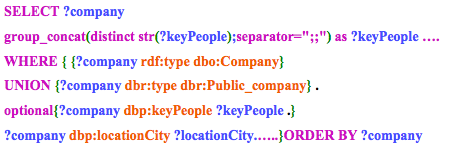
\includegraphics[width=10cm]{DB_Com}
	\caption[DBpedia query for companies]{DBpedia query for companies}
	\label{fig:db}
	\end{center}
\end{figure}

\subsubsection{Freebase: Companies}
Freebase provides a web service to query entities and returns them in a JSON format. The total number of entities returned by our query is 3,182. Similar to the SPARQL query above we decided to make some attributes optional while others are non-optional. Specifically, the \texttt{number\_of\_employees} is non-optional because we use it to compare companies in each dataset and to reduce the number of companies down from 230,000. To make sure we receive the right attributes we first tested queries on the query page. To actually retrieve the data we used Java to make calls to the MQL Read API\footnote{https://developers.google.com/freebase/v1/mqlread?hl=en}. To avoid issues during the mapping procedure in MapForce we concatenated attributes with multiple values with a delimiter. 

\begin{figure}[H]
	\begin{center}
	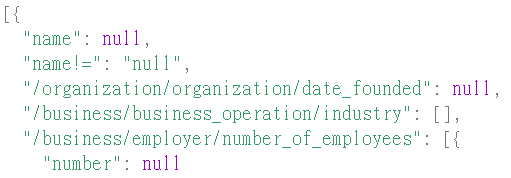
\includegraphics[width=9cm]{Freebase_query}
	\caption[Freebase query for companies]{Freebase query for companies}
	\label{fig:db}
	\end{center}
\end{figure}

\subsubsection{DBpedia: Locations}
%Silvia/Zehui
We extracted information about locations from DBpedia using the same method as for companies. Similarly, we limited the resource type in our SPARQL query to \texttt{City} and \texttt{AdministrativeRegion}, which are more relevant to our company dataset. We also found the same problem of many values for attributes without any extra provenance information, whch makes identifying the current state hard. As such we used the maximum number for \texttt{population}, for example. Lastly, the names of the locations are often provided in different languages in DBpedia. Because we focused on English in our project we chose the value for \texttt{name} by filtering the language labels accordingly. 

















